%!TEX TS-program = xelatex
\documentclass[a4paper,14pt]{article}


%%% Работа с русским языком
\usepackage[english,russian]{babel}   %% загружает пакет многоязыковой вёрстки
\usepackage{fontspec}      %% подготавливает загрузку шрифтов Open Type, True Type и др.
\defaultfontfeatures{Ligatures={TeX},Renderer=Basic}  %% свойства шрифтов по умолчанию
\setmainfont[Ligatures={TeX,Historic}]{Times New Roman} %% задаёт основной шрифт документа
\setsansfont{Comic Sans MS}                    %% задаёт шрифт без засечек
\setmonofont{Courier New}
\usepackage{indentfirst}
\frenchspacing

\renewcommand{\epsilon}{\ensuremath{\varepsilon}}
\renewcommand{\phi}{\ensuremath{\varphi}}
\renewcommand{\kappa}{\ensuremath{\varkappa}}
\renewcommand{\le}{\ensuremath{\leqslant}}
\renewcommand{\leq}{\ensuremath{\leqslant}}
\renewcommand{\ge}{\ensuremath{\geqslant}}
\renewcommand{\geq}{\ensuremath{\geqslant}}
\renewcommand{\emptyset}{\varnothing}

%%% Дополнительная работа с математикой
\usepackage{amsmath,amsfonts,amssymb,amsthm,mathtools} % AMS
\usepackage{icomma} % "Умная" запятая: $0,2$ --- число, $0, 2$ --- перечисление

%% Номера формул
%\mathtoolsset{showonlyrefs=true} % Показывать номера только у тех формул, на которые есть \eqref{} в тексте.
%\usepackage{leqno} % Нумерация формул слева	

%% Перенос знаков в формулах (по Львовскому)
\newcommand*{\hm}[1]{#1\nobreak\discretionary{}
	{\hbox{$\mathsurround=0pt #1$}}{}}

%%% Работа с картинками
\usepackage{graphicx}  % Для вставки рисунков
\graphicspath{{images/}}  % папки с картинками
\setlength\fboxsep{3pt} % Отступ рамки \fbox{} от рисунка
\setlength\fboxrule{1pt} % Толщина линий рамки \fbox{}
\usepackage{wrapfig} % Обтекание рисунков текстом

%%% Работа с таблицами
\usepackage{array,tabularx,tabulary,booktabs} % Дополнительная работа с таблицами
\usepackage{longtable}  % Длинные таблицы
\usepackage{multirow} % Слияние строк в таблице
\usepackage{float}% http://ctan.org/pkg/float

%%% Программирование
\usepackage{etoolbox} % логические операторы


%%% Страница
\usepackage{extsizes} % Возможность сделать 14-й шрифт
\usepackage{geometry} % Простой способ задавать поля
\geometry{top=20mm}
\geometry{bottom=20mm}
\geometry{left=20mm}
\geometry{right=10mm}
%
%\usepackage{fancyhdr} % Колонтитулы
% 	\pagestyle{fancy}
%\renewcommand{\headrulewidth}{0pt}  % Толщина линейки, отчеркивающей верхний колонтитул
% 	\lfoot{Нижний левый}
% 	\rfoot{Нижний правый}
% 	\rhead{Верхний правый}
% 	\chead{Верхний в центре}
% 	\lhead{Верхний левый}
%	\cfoot{Нижний в центре} % По умолчанию здесь номер страницы

\usepackage{setspace} % Интерлиньяж
\onehalfspacing % Интерлиньяж 1.5
%\doublespacing % Интерлиньяж 2
%\singlespacing % Интерлиньяж 1

\usepackage{lastpage} % Узнать, сколько всего страниц в документе.

\usepackage{soul} % Модификаторы начертания

\usepackage{hyperref}
\usepackage[usenames,dvipsnames,svgnames,table,rgb]{xcolor}
\hypersetup{				% Гиперссылки
	unicode=true,           % русские буквы в раздела PDF
	pdftitle={Разработка программной системы для автоматической генерации графа диалогов по текстам пьес.},   % Заголовок
	pdfauthor={Подчезерцев А.Е.},      % Автор
	pdfsubject={ВКР},      % Тема
	pdfcreator={Подчезерцев А.Е.}, % Создатель
	pdfproducer={Подчезерцев А.Е.}, % Производитель
	pdfkeywords={keyword1} {key2} {key3}, % Ключевые слова
	colorlinks=true,       	% false: ссылки в рамках; true: цветные ссылки
	linkcolor=black,          % внутренние ссылки
	citecolor=black,        % на библиографию
	filecolor=magenta,      % на файлы
	urlcolor=black           % на URL
}
\makeatletter 
\def\@biblabel#1{#1. } 
\makeatother
\usepackage{cite} % Работа с библиографией
%\usepackage[superscript]{cite} % Ссылки в верхних индексах
%\usepackage[nocompress]{cite} % 
\usepackage{csquotes} % Еще инструменты для ссылок

\usepackage{multicol} % Несколько колонок

\usepackage{tikz} % Работа с графикой
\usepackage{pgfplots}
\usepackage{pgfplotstable}

\usepackage{ dsfont }

\newcommand{\imref}[1]{рис.~\ref{#1}}

\usepackage{spreadtab}
\newcolumntype{K}[1]{@{}>{\centering\arraybackslash}p{#1cm}@{}}


\usepackage{xparse}
\usepackage{fancyvrb}

\RecustomVerbatimCommand{\VerbatimInput}{VerbatimInput}
{
	fontsize=\footnotesize    
}

\newcolumntype{?}[1]{!{\vrule width #1}}

\usepackage{tocloft}
\renewcommand{\cftsecleader}{\cftdotfill{\cftdotsep}}

\usepackage{pdfpages}

\usepackage{rotating}

\usepackage{pdflscape}

\usepackage{ragged2e}
\usepackage{microtype}

% Выравнивание по ширине без переносов слов
\justifying
\sloppy
\tolerance=500
\hyphenpenalty=10000
\emergencystretch=3em

% Подогнать таблицу под ширину страницы
\usepackage{adjustbox}

\usepackage{titlesec}

% ГОСТ заголовки таблицы
\usepackage[font=small]{caption}

\captionsetup[figure]{justification=centering,labelsep=period} % Картинки по центру, с точкой после рис

\DeclareCaptionLabelFormat{rightline}{\rightline{\bothIfFirst{#1}{ }#2}}
\captionsetup[table]{justification=centering,labelformat=rightline,labelsep=newline}

\newcommand{\tablecaption}[1]{\addtocounter{table}{1}\small \begin{flushright}\tablename \ \thetable\end{flushright}%	
	\begin{center}#1\end{center}}

\usepackage{enumerate}
\begin{document} 	
	
\begin{titlepage}
	\begin{center}
 		ФЕДЕРАЛЬНОЕ  ГОСУДАРСТВЕННОЕ АВТОНОМНОЕ \\
		ОБРАЗОВАТЕЛЬНОЕ УЧРЕЖДЕНИЕ ВЫСШЕГО ОБРАЗОВАНИЯ\\
		«НАЦИОНАЛЬНЫЙ ИССЛЕДОВАТЕЛЬСКИЙ УНИВЕРСИТЕТ\\
		«ВЫСШАЯ ШКОЛА ЭКОНОМИКИ»
	\end{center}
	
	\begin{center}
		\textbf{Московский институт электроники и математики}
		
		\textbf{им. А.Н.Тихонова НИУ ВШЭ}
		
		\vspace{2ex}
		
		\textbf{Департамент компьютерной инженерии}
	\end{center}
	\vspace{1ex}	
	
	\begin{center}
		Курс «Системное проектирование цифровых устройств»
	\end{center}	
	
	
	\begin{center}
	\textbf{ОТЧЕТ\\
		ПО ЛАБОРАТОРНОЙ РАБОТЕ №1
	}
	\end{center}	

	\begin{center}
		Тема работы: «Разработка и программирование Soft-процессорных ядер с архитектурой однотактный MIPS. Часть 1»
	\end{center}

	\vspace{2ex}

	\begin{flushright}
		\textbf{Выполнили:}
		
		\vspace{2ex}
		
		Студенты группы БИВ174
		
		Бригада №5
		
		\vspace{2ex}
		
		Подчезерцев Алексей Евгеньевич
		
		Солодянкин Андрей Александрович
		\vspace{2ex}
		
		\textbf{Принял:}
		
		асс. МИЭМ НИУ ВШЭ
		
		Американов А.А.
		
	\end{flushright}

	\vfill
	\begin{center}
		Москва \the\year \, г.
	\end{center}
	
\end{titlepage}
\addtocounter{page}{1}
	
\section*{\normalsize \hfill Аннотация \hfill}

\sloppy

\begin{center}
	A Software Tool for Automatic Generation of a Graph of Conversation Using a Drama Corpus
\end{center}
\section*{\normalsize \hfill Abstract \hfill}


\newpage

\tableofcontents
\pagebreak

\section*{Введение}
\addcontentsline{toc}{section}{\protect\numberline{}Введение}


В последние годы технологии машинного обучения стали неотъемлемой частью нашей жизни. 
Они представлены голосовыми помощниками, рекомендательными системами, умными домами, умными автомобилями и другими системами.
Важной частью этих систем являются модули, которые помогают сделать понятным для компьютера то, что от него требуется.
Для систем по обработке текста это модули обработки естественного языка или Natural Language Processing (NLP).

Компьютер без дополнительной помощи не способен обрабатывать естественный текст, зато компьютер хорошо работает с числами.
Поэтому для того, чтобы <<подружить>> вычислительную машину с текстом, нужно представить текст в виде чисел или в виде многомерных векторов.
Эти вектора также называют эмбеддингами.

Модели, использующие данный принцип, называются моделями векторного представления слов.
В основе большей части данных моделей лежит гипотеза дистрибутивности [9].
Эта гипотеза заключается в том, что слова со схожим смыслом встречаются в похожих контекстах.

Прорывной и наиболее известной моделью векторного представления слов является выпущенная в 2013 году модель word2vec [6].
Было представлено две архитектуры модели нейронной сети word2vec: Continuous Bag-of-Words
(CBOW) и Skip-gram. 
Continuous Bag-of-Words дословно переводится как <<непрерывный мешок слов>>.
Работает архитектура похожим образом, предсказывается вероятность появления слова по его контексту в виде окна фиксированного размера.
Архитектура Skip-gram наоборот предсказывает вероятность появления контекста у заданного слова.
Порядок слов в контексте не влияет на результат ни в одном из этих алгоритмов.
В процессе обучения модель корректирует веса между входным и скрытым слоем, которые в дальнейшем станут эмбеддингами слов.

Оказалось, что полученные векторные представления слов скрывают в себе семантические отношения между словами.
Это хорошо заметно на примере задачи по построению пропорциональной аналогии.
Эту задачу можно сформулировать так: <<какое слово \textit{d} относится к слову \textit{c} так, 
как слово \textit{b} относится к слову \textit{a}>>.
В модели word2vec это отношение можно выразить в виде разницы векторов.
Для слов \textit{a} и \textit{b} с соответствующими им векторами $v_a$ и $v_b$ вектор разности $v_a - v_b$ будет характеризовать семантическую связь между словами.
Тогда для решением задачи пропорциональной аналогии будет выражение $v_d - v_c = v_b - v_a$, где $v_d$ и $v_c$ эмбеддинги слов \textit{d} и \textit{c} соответственно.

Из полученного выражения получаем: $v_d = v_c + v_b - v_a$.
Но вероятность того, что полученный вектор $v_d$ совпадает с вектором какого-либо слова крайне мала, поэтому в качестве ответа берется слово с вектором наиболее близким к $v_d$, формула (\ref{solv_prop}).

\begin{equation}
	v_d = \underset{v'}{argmax} \cos (v', v_c + v_b - v_a)
	\label{solv_prop}
\end{equation}

Данная задача для модели word2vec исследовалась в работе []. Где пришли к выводу, что эта модель не всегда дает правильный ответ для задачи пропорциональной аналогии.

В настоящее время появляется все больше моделей для обработки естественного языка.

В 2017 году в исследовании [] была предложена модель контекстуализированной модели обработки естественного языка ELMo (Embeddings from Language Models).
Если в модели word2vec векторное представление слов было одним и тем же независимо от контекста, то в ELMo решается эта проблема.
Для каждого контекста будет свой эмбеддинг.
В основе архитектуры ELMo лежат блоки долгой краткосрочной памяти (LSTM - Long Short-Term Memory).
Данные блоки расположены в прямом и обратном направлениях для того, чтобы при создании эмбеддинга учитывался контекст до и после слова.

Вскоре после выхода ELMo вышла модель BERT или Bidirectional Encoder Representations from Transformers.
BERT – это модель, побившая несколько рекордов по успешности решения ряда NLP-задач, например BERT показала лучшее качество на тесте SQuAD 1.1 [5].
BERT также контекстуализированная модель.
Архитектура модели BERT представляет из себя последовательность двунаправленных кодировщиков из Transformer.
В основе обучения модели лежат две идеи:

\begin{enumerate}
	\itemsep0em 
	\item Первая состоит в том, чтобы заменить 15\% текста масками и заставить модель предсказывать пропущенные слова.
	\itemsep0em 
	\item Вторая идея заключается в том, чтобы научить модель оценивать насколько одно предложение является логичным продолжением второго.
\end{enumerate}

Успех модели, помимо хорошего качества, можно объяснить тем, что код модели был выложен в открытый доступ, а также были выложены различные модели, предобученные на больших объемах данных.
Это дало возможность всем разработчикам встроить модель BERT в свои модели машинного обучения для обработки естественного языка.
%Вскоре после выхода статьи, описывающей модель, команда разработчиков также выложила в открытый доступ код модели и сделала возможным скачивание различных версий BERT, которые уже были предобучены на больших наборах данных.
%Этот знаменательный шаг позволил любому разработчику встраивать в свои модели машинного обучения для обработки естественного языка уже готовый мощный компонент, сохраняя свои время, энергию и ресурсы, необходимые для обучения модели обработки языка с нуля.
%Среди них можно выделить две модели ELMO и BERT.

ELMo и BERT - контекстуализированные модели, это значит, что векторное представление одного и того же слова будет отличаться в зависимости от его контекста.
Отсюда возникает вопрос, возможно ли провести аффинные преобразования в семантическом пространстве модели BERT?

\textbf{Целью} данной практики является исследование аффинных преобразований для модели BERT и определение точности этих преобразований.

Для достижения поставленной цели потребовалось решить следующие \textbf{задачи}:

\begin{enumerate}
	\itemsep0em 
	\item Исследование моделей векторного представления слов;
		\itemsep0em 
	\item Исследование методов оценки аффинных преобразований;
		\itemsep0em 
	\item Разработка метода оценки точности параллельного переноса для контекстуализированных моделей;
		\itemsep0em 
	\item Подготовка экспериментальных данных;
		\itemsep0em 
	\item Проведение экспериментов;
		\itemsep0em 
	\item Оценка полученных результатов.

\end{enumerate}

\newpage


\section{Обзор литературы}

\subsection{Появления моделей векторных представлений слов}

Векторное представление слов является одним из ключевых инструментов в обработке естественного языка.
Основная идея заключается в том, чтобы сопоставить каждому слову вектор определенной величины.

Самой простой реализацией модели векторного представления слов является one-hot encoding.
Идея этой модели заключается в том, что в наборе из \textit{K} слов каждому слову $k_i$ сопоставить вектор $v_i$ длиной \textit{K} со всеми нулями и одной единицей в позиции \textit{i}, где \textit{i} - это номер слова во всем наборе (\ref{fraq:one-hot}).

\begin{equation}
	v_i^j = \left\{
	\begin{matrix}
		& 1, i = j\\
		& 0, i \neq j
	\end{matrix}
	\right.
	,\;j = 1, ..., K	
	\label{fraq:one-hot}
\end{equation}

Недостатком этого метода является то, что по данным векторным представлениям нельзя судить о семантической схожести слов.
Также для при обработке реальных текстов размер словаря будет очень большим, а значит длина векторных представлений будет очень большой, данные вектора неэффективно хранить в памяти.
Также к многих алгоритмов машинного обучения могут возникнуть сложности с обработкой разреженных векторов.

Позднее появились более продвинутые модели векторного представления.
В этих реализациях уже наблюдаются семантические отношения между эмбеддингами слов.
Модели векторного представления делятся на две группы в зависимости от используемых методов.

Первая группа - статистические модели векторного представления.
При работе этих моделей строится матрица совместной встречаемости слов, далее эта матрица подвергается сингулярному разложению.
Одна из полученных после разложения матриц содержит вектора слов.

%Первая группа включает в себя методы, использующие статистики корпуса текста. 
%Они основываются на построении матрицы � совместной встречаемости слов
%(cooccurrence matrix), к которой впоследствии применяют сингулярное разложение 
%(singular value decomposition, SVD). Одна из матриц, получаемых в результате 
%сингулярного разложения, содержит вектора слов. Такой подход используется в 
%латентно-семантическом анализе (latent semantic analysis, LSA), где строится матрица 
%встречаемости слов в документах

Вторая группа - предиктивными модели.
Данные модели для создания эмбеддинга используют контекст, используются слова, попадающие в окно определенного размера вокруг интересующего нас слова.
Для работы используются нейронные сети.
%Вторая группа включает в себя предиктивные модели, использующие 
%информацию о локальном окружении слова – его контексте. Здесь под контекстом 
%понимают окно заданного размера. Такие модели основаны на нейронных сетях, 
%которые обучаются на неразмеченном корпусе текстов. Чаще всего понятие 
%«эмбеддинги» связывают именно с предиктивными моделями

В данный момент большей популярностью пользуются предиктивные модели.
Большая популярность пришла к этим моделям с появлением word2vec.

\subsection{Word2vec}
	
	Идея создания векторов в word2vec основана на предположении о контекстной близости, а именно на том, что слова встречающиеся в одинаковых контекстах скорее всего имеют схожее значение.
	
	Модель word2vec является простейшей нейронной сетью с обратным распространением ошибки.
	у нее один скрытый слой.
	В основе обучения модели лежит идея, что тренировать можно не только на контексте из предыдущих слов, но также использовать слова, после целевого слова.
	При этом порядок слов в контексте не учитывается.

	
\begin{comment}
Предлагается проверять схожесть слов при помощи косинусного сходства их векторных представлений (\ref{eq:cos_sim}).

\begin{equation}
	similarity(A,B) = cos(A,B) = cos(\theta) = \dfrac{A\cdot B}{\|A\| \|B\|}
	\label{eq:cos_sim}
\end{equation}

где

$A$ - векторное представление первого слова,

$B$ - векторное представление второго слова,

$\theta$ - угол между векторами $A$ и $B$.

\end{comment}

Существует 2 метода обучения word2vec: CBOW (Continuous Bag of Words) и  Skip-gram.
Основная цель архитектуры Continuous Bag-of-Word состоит в том, чтобы предсказать пропущенное слово по его контексту.
В Skip-gram предсказывается контекст по целевому слову.
%В Skip-gram по слову прогнозируется слова из его контекста, в CBOW, наоборот, по контексту предсказывается слово.
%В качестве выходного слоя в моделях применяется функция softmax в различных вариациях для того.

На рисунке \ref{fig:word2vec} представлены изображения архитектур CBOW и Skip-gram.
Где $V$ -- мощность словаря, $x$ -- слова, подающиеся на вход нейронной сети, закодированные методом one-hot encoding (\ref{fraq:one-hot}) для словаря мощностью $V$, $N$ -- количество нейронов в скрытом слое и $y$ -- результат работы функции активации softmax.

\begin{figure}[H]
	\begin{minipage}[h]{0.49\linewidth}
		\center{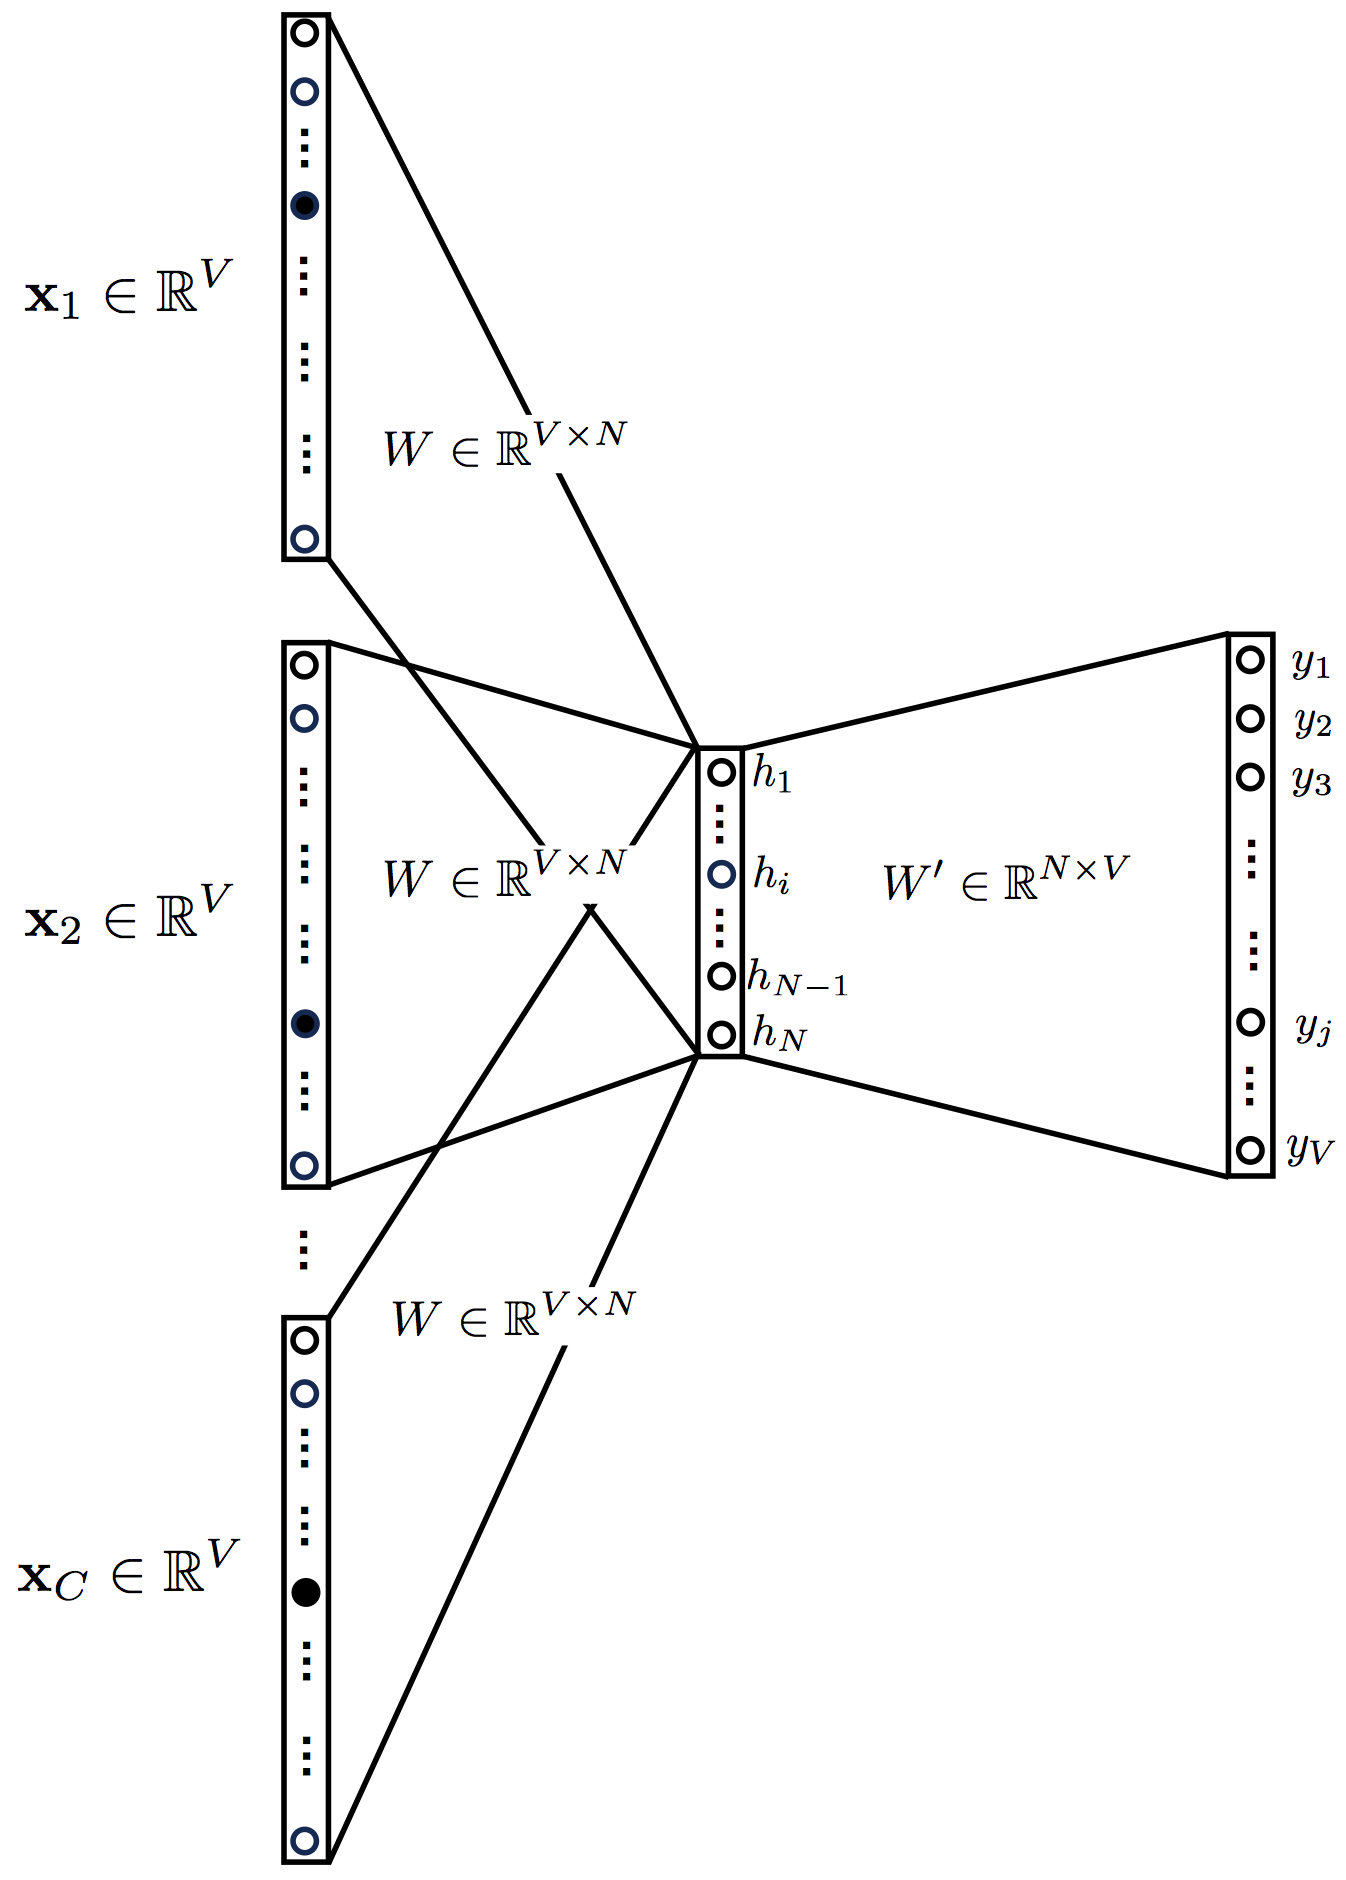
\includegraphics[width=0.85\linewidth]{image/Cbow} \\ а)}
	\end{minipage}
	\hfill
	\begin{minipage}[h]{0.49\linewidth}
		\center{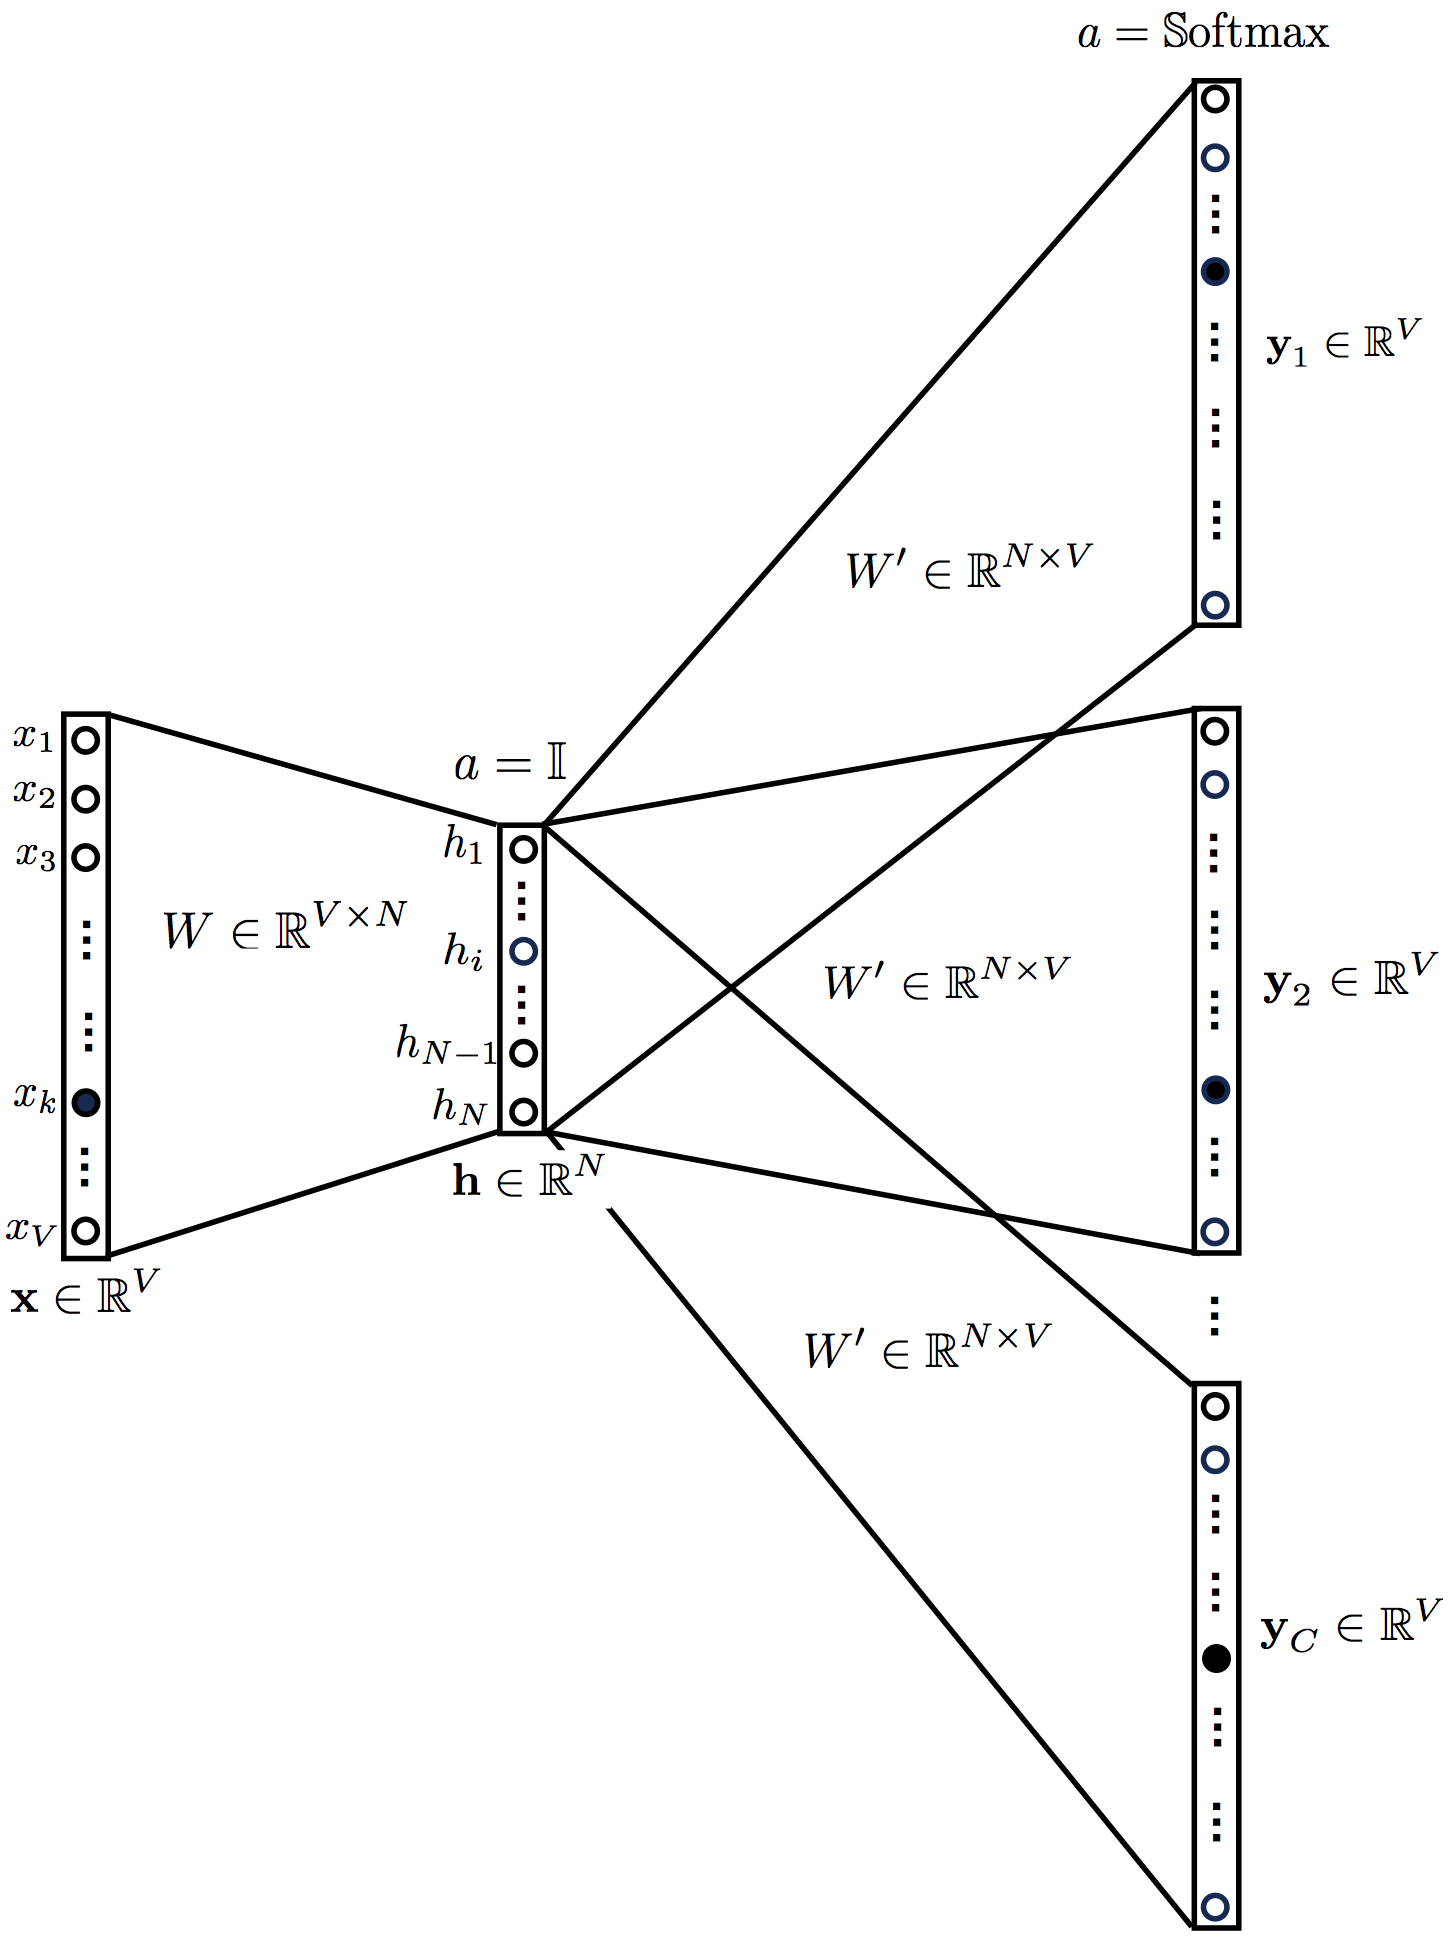
\includegraphics[width=0.85\linewidth]{image/Skip-gram} \\ б)}
	\end{minipage}
	\caption{Схемы архитектур CBOW (a), Skip-gram (б)}
	\label{fig:word2vec}
\end{figure}

Архитектуры представляют из себя полносвязные нейронные сети с обратным распространением ошибки.
Для больших словарей метод активации softmax накладывает серьезные вычислительные нагрузки.
Поэтому для оптимизации было предложено использовать метод негативного семплирования (negative sampling).

При работе softmax каждое слово  представляет из себя отдельный класс, авторы word2vec предложили использовать бинарную классификацию вместо многоклассовой.
Предлагается научить модель отличать пары слов, которые встречаются в одном контексте, от тех, которые никогда не стоят в одном контексте.

Появление модели word2vec послужило мощным толчком для развития моделей обработки естественного языка.

%Continuous Bag-of-Words дословно переводится как <<непрерывный мешок слов>>.
%Работает архитектура похожим образом, предсказывается вероятность появления слова по его контексту в виде окна фиксированного размера.
%Архитектура Skip-gram наоборот предсказывает вероятность появления контекста у заданного слова.
%Порядок слов в контексте не влияет на результат ни в одном из этих алгоритмов.
%В процессе обучения модель корректирует веса между входным и скрытым слоем, которые в дальнейшем станут эмбеддингами слов.

\subsection{FastText}

FastText является продолжением развития модели word2vec.
FastText имеет архитектуру Skip-gram.
При этом в fastText отличается от word2vec тем, что у новой модели используются N-граммы символов.
Например, для слова молоко 3-граммами являются <мо, мол, оло, лок, око, ко>, где символы << < >> и << > >> кодируют начало и конец слова соответственно.
Векторные представления строятся именно для N-грамм, векторные представления слов - это сумма векторных представлений всех его N-грамм.
При этом решается проблема того, что словарь модели word2vec был ограничен и не все формы слов вошли в словарь.
Также, использование N-грамм позволяет получать векторные представления для редких слов.

В русском языке существуют слова омонимы и омографы, слова, которые совпадают в написании, но имеют разный смысл.
Предыдущие методы обработки естественного языка никак не решали эту проблему.
Одной из первых эту проблему постаралась решить модель ELMo.

\subsection{ELMo}

ELMo (Embeddings from Language Models) -- модель обработки естественного языка, которая представляет собой двунаправленную рекуррентную нейронную сеть с LSTM.
модель была предложена в работах [].
Модель учитывает семантическую неоднозначность слов в предложениях, и эмбеддинги, присваиваемые словам, зависят не только от самого слова, но и от контекста.
Основная идея получения эмбеддингов -- использование скрытых состояний LSTM.
Разберемся по подробнее с LSTM блоками.

\subsubsection{LSTM}

LSTM или Long short-term memory дословно переводится как долгая краткосрочная память, были предложены в статье [].
Данные блоки являются разновидностью архитектуры рекуррентных нейронных сетях и предназначены для того, чтобы хранить информацию на длинные и на короткие промежутки времени.

Данные блоки имеют одну особенность, в них нет функции активации.
За счет этого хранимая информация не размываются по времени и во время обучения при использовании метода обратного распространения ошибки вычисляемый градиент не исчезает.

В LSTM модуле есть 2 основных компонента: состояние ячейки и различные фильтры.
Состояние ячейки -- это память сети, которая передается по всей цепочке.

Во время обучения состояние ячейки постоянно меняется. Происходит добавление и удаление информации.
Все это контролируют фильтры.
Фильтры состоят из сигмоидальной нейронной сети и операции поточечного умножения.
Сигмоидальный модуль возвращает числа в диапазоне [0;1], которые обозначают долю блока информации, которую следует пропустить дальше по сети.
Фильтры бывают трех типов:
\begin{enumerate}
	\itemsep0em 
	\item Забывания;
	\itemsep0em 
	\item Входные;
	\itemsep0em 
	\item Выходные.
\end{enumerate}

На рисунке \ref{fig:LSTM_layers}.а изображен фильтр забывания.
На данном этапе решается какую информацию можно забыть или оставить.
$h_{t-1}$ -- значения выхода из предыдущего блока, $x_t$ -- вход данного блока.
Данные значения проходят обработку в сигмоидальном блоке.
Результаты находятся в диапазоне [0;1] то, что ближе к 0 будет забыто, что ближе к 1 оставлено (\ref{fraq:forget}).


\begin{equation}
	f_t = \sigma(W_f\cdot[h_{t-1},x_t] + b_f)
	\label{fraq:forget}
\end{equation}

На рисунке \ref{fig:LSTM_layers}.б решается какая информация будет храниться в состоянии ячейки.
Сигмоидальный блок решает какую информацию необходимо обновить (\ref{fraq:enter_sigma_i}), tanh-слой строит вектор со значениями, которые могут быть добавлены в состояние ячейки (\ref{fraq:enter_sigma}). 

\begin{equation}
	i_t = \sigma(W_i\cdot[h_{t-1},x_t] + b_i) 
	\label{fraq:enter_sigma_i}
\end{equation}
\begin{equation}
	\tilde C_t = \tanh(W_C\cdot[h_{t-1},x_t] + b_C)
	\label{fraq:enter_sigma}
\end{equation}

На рисунке \ref{fig:LSTM_layers}.в проиллюстрирован процесс изменения состояния ячейки.
Ненужная информация в $C_{t-1}$ забывается после умножения на $f_t$.
Затем к состоянию ячейки добавляются текущие изменения $i_t * \tilde C_t$.
Все вместе можно записать формулой (\ref{fraq:changes_sigma}).

\begin{equation}
	\tilde C_t = f-t * C_{t-1} + i_t * \tilde C_t
	\label{fraq:changes_sigma}
\end{equation}



\begin{figure}[H]
	\begin{minipage}[h]{0.4\linewidth}
		\center{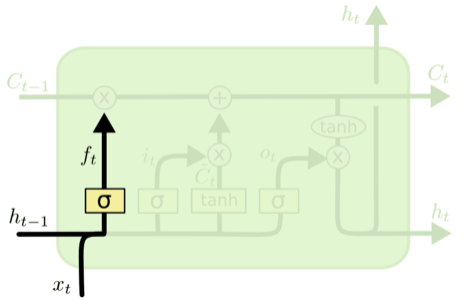
\includegraphics[width=1\linewidth]{image/LSTM_1}} а) \\
	\end{minipage}
	\hfill
	\begin{minipage}[h]{0.4\linewidth}
		\center{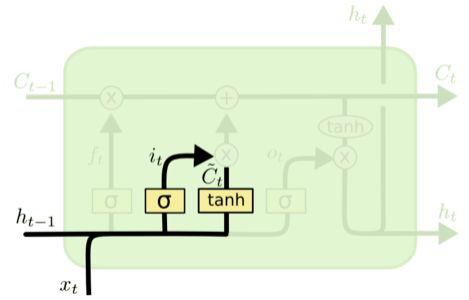
\includegraphics[width=1\linewidth]{image/LSTM_2}} \\б)
	\end{minipage}
	\vfill
	\begin{minipage}[h]{0.4\linewidth}
		\center{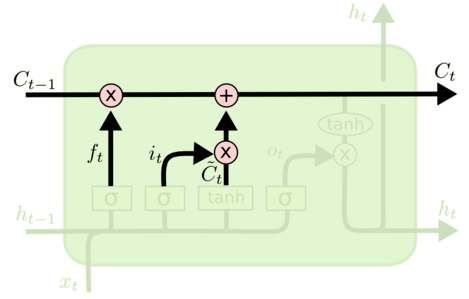
\includegraphics[width=1\linewidth]{image/LSTM_3}} в) \\
	\end{minipage}
	\hfill
	\begin{minipage}[h]{0.4\linewidth}
		\center{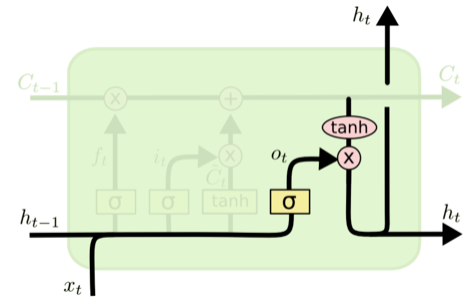
\includegraphics[width=1\linewidth]{image/LSTM_4}} г) \\
	\end{minipage}
	\caption{Виды фильтров: 
		 a) слой фильтра забывания,
		 b) слой входного фильтра,
		 c) применение текущих изменений,
		 d) слой выходного фильтра.}
	\label{fig:LSTM_layers}
\end{figure}

На рисунке \ref{fig:LSTM_layers}.г изображен финальный формирования выходов.
Сначала в сигмоидальном слое поступает информация предыдущего выхода $h_{t−1}$ и текущего входа $x_t$, где определятся какая информация из состояния ячейки будет отправлена на выход (\ref{fraq:out_sigma_o}).
Далее значения из состояния ячейки обрабатываются tanh-слоем и перемножаются со значениями с сигмоидального слоя (\ref*{fraq:out_sigma}).

\begin{equation}
	o_t = \sigma(W_o\cdot[h_{t-1},x_t]) 
	\label{fraq:out_sigma_o}
\end{equation}
\begin{equation}
	\tilde h_t = o_t * \tanh(C_t)
	\label{fraq:out_sigma}
\end{equation}

После преобразований $h_t$ и $C_t$ передаются на следующий блок по цепочке.	

\subsubsection{Структура ELMo}

Архитектура ELMo представлена на рисунке \ref{fig:elmostructure}.а.
ELMo состит из двух двухслойных разнонаправленных рекуррентных LSTM сетей.
Было замечено, что верхние слои LSTM сети отвечают за семантический смысл слова, а нижние -- за синтаксис и грамматику.

\begin{figure}[H]
	\begin{minipage}[h]{0.499\linewidth}
		\center{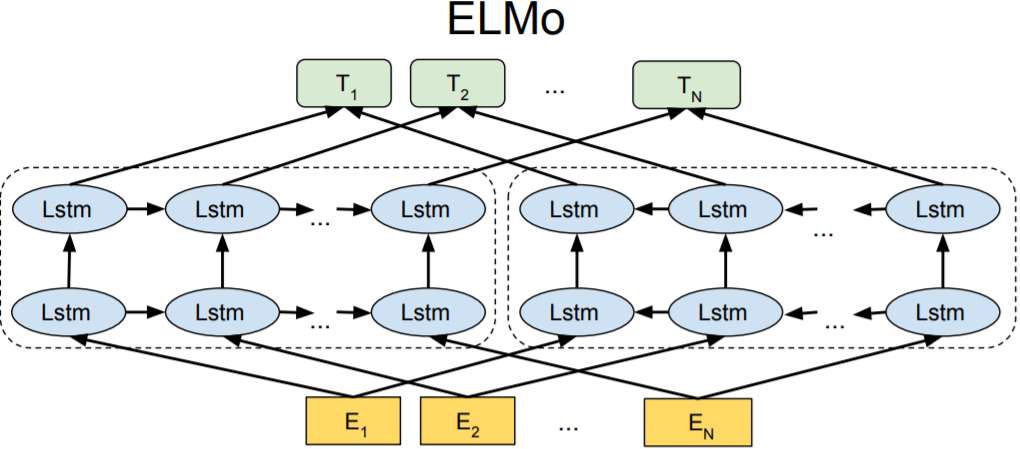
\includegraphics[width=1\linewidth]{image/elmo_structure} \\ а)}
	\end{minipage}
	\hfill
	\begin{minipage}[h]{0.499\linewidth}
		\center{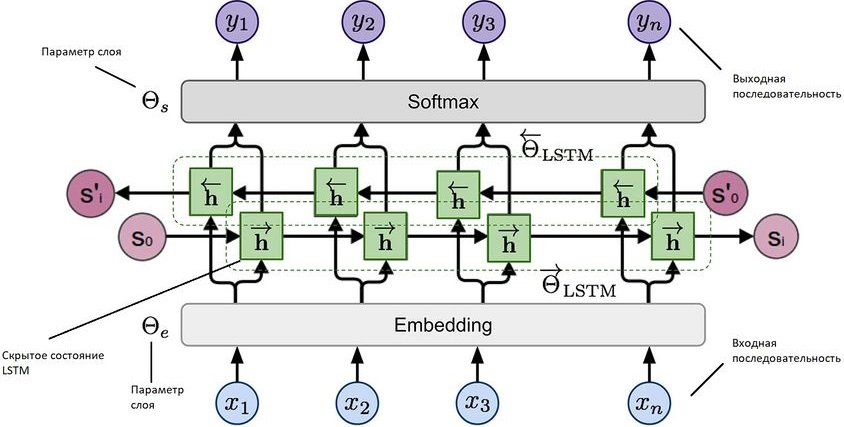
\includegraphics[width=1\linewidth]{image/900px-ElmoExplain} \\ б)}
	\end{minipage}
	\caption{Архитектура модели ELMo (а), принцип работы модели ELMo (б)}
	\label{fig:elmostructure}
\end{figure}

На рисунке \ref{fig:elmostructure}.б схематично изображен принцип работы модели ELMo.
Пусть на вход подаются токены $t_1, ...., t_N$, на которые разделено предложение.
Будем считать логарифм правдоподобия метки слова в обоих направлениях, учитывая контекст справа и слева от слова.
так модель предсказывает вероятность следующего токена с учетом истории.

Пусть есть $L$ слоев сети, входные и выходные данные представляются в виде векторных представлений слов.
Каждый результирующий вектор будет считаться на основании множества (\ref{fraq:array_elmo}).

\begin{equation}
	\left\{ x_k^{LM}, \overrightarrow{h_{k,j}^{LM}}, \overleftarrow{h_{k,j}^{LM}}  |j = 1, ...,L\right\} = 
	\left\{h_{k,j}^{LM}|j = 1, ...,L
	\right\}
	\label{fraq:array_elmo}
\end{equation}

где $x_k^{LM}$ -- входящий токен, $\overrightarrow{h_{k,j}^{LM}}, \overleftarrow{h_{k,j}^{LM}}$ -- скрытые слои в обоих направлениях.

Результатом работы ELMo будет выражение (\ref{fraq:elmo_result}).

\begin{equation}
	ELMO_k^{task} = \gamma^{task}\sum_{j=0}^{L} s_{i}^{task}h_{k,j}^{LM}
	\label{fraq:elmo_result}
\end{equation}

где $\gamma^{task}$ -- масштабирующий коэффициент, который регулирует то, как могут отличаться по норме ембеддинги слов, $s_{i}^{task}$ -- обучаемые параметры, нормализованные функцией softmax.

Векторным представлением слова будет яаляться взвешенная сумма значений на всех скрытых слоях ELMo.

Вскоре после выхода ELMo появилась еще одна мощная контекстуализированная модель, называется она BERT.

\subsection{BERT}



\subsection{Выводы}

\newpage

\section{Теоретическая часть}
\subsection{Выводы}
\begin{enumerate}
	\itemsep0em 
	\item 
\end{enumerate}

\newpage
\section{Практическая часть}

\subsection{Выводы}
\begin{enumerate}
	\itemsep0em 
	\item 
\end{enumerate}

\newpage
\section{Заключение}

\newpage 
\renewcommand{\refname}{{\normalsize \hfill Список использованных источников \hfill}} 
\bibliographystyle{unsrt}
\begin{thebibliography}{30}
	\addcontentsline{toc}{section}{Список использованных источников} 
% Введение
\bibitem{infro1}

\end{thebibliography}

\newpage



\end{document}